\documentclass{article}

\usepackage{fancyhdr}
\usepackage{extramarks}
\usepackage{amsmath}
\usepackage{amsthm}
\usepackage{amsfonts}
\usepackage{tikz}
\usepackage[plain]{algorithm}
\usepackage{algpseudocode}
\usepackage{mathtools}
\usepackage{graphicx}
\graphicspath{ {./images/} }

\DeclarePairedDelimiter\abs{\lvert}{\rvert}%
\DeclarePairedDelimiter\norm{\lVert}{\rVert}%

\makeatletter
\let\oldabs\abs
\def\abs{\@ifstar{\oldabs}{\oldabs*}}
%
\let\oldnorm\norm
\def\norm{\@ifstar{\oldnorm}{\oldnorm*}}
\makeatother

\newcommand*{\Value}{\frac{1}{2}x^2}%

\usetikzlibrary{automata,positioning}

%
% Basic Document Settings
%

\topmargin=-0.45in
\evensidemargin=0in
\oddsidemargin=0in
\textwidth=6.5in
\textheight=9.0in
\headsep=0.25in

\linespread{1.1}

\pagestyle{fancy}
\lhead{\hmwkAuthorName}
\chead{\hmwkClass\ (\hmwkClassInstructor\ \hmwkClassTime): \hmwkTitle}
\rhead{\firstxmark}
\lfoot{\lastxmark}
\cfoot{\thepage}

\renewcommand\headrulewidth{0.4pt}
\renewcommand\footrulewidth{0.4pt}

\setlength\parindent{0pt}

%
% Create Problem Sections
%

\newcommand{\enterProblemHeader}[1]{
    \nobreak\extramarks{}{Problem \arabic{#1} continued on next page\ldots}\nobreak{}
    \nobreak\extramarks{Problem \arabic{#1} (continued)}{Problem \arabic{#1} continued on next page\ldots}\nobreak{}
}

\newcommand{\exitProblemHeader}[1]{
    \nobreak\extramarks{Problem \arabic{#1} (continued)}{Problem \arabic{#1} continued on next page\ldots}\nobreak{}
    \stepcounter{#1}
    \nobreak\extramarks{Problem \arabic{#1}}{}\nobreak{}
}

\setcounter{secnumdepth}{0}
\newcounter{partCounter}
\newcounter{homeworkProblemCounter}
\setcounter{homeworkProblemCounter}{1}
\nobreak\extramarks{Problem \arabic{homeworkProblemCounter}}{}\nobreak{}

%
% Homework Problem Environment
%
% This environment takes an optional argument. When given, it will adjust the
% problem counter. This is useful for when the problems given for your
% assignment aren't sequential. See the last 3 problems of this template for an
% example.
%
\newenvironment{homeworkProblem}[1][-1]{
    \ifnum#1>0
        \setcounter{homeworkProblemCounter}{#1}
    \fi
    \section{Problem \arabic{homeworkProblemCounter}}
    \setcounter{partCounter}{1}
    \enterProblemHeader{homeworkProblemCounter}
}{
    \exitProblemHeader{homeworkProblemCounter}
}

%
% Homework Details
%   - Title
%   - Due date
%   - Class
%   - Section/Time
%   - Instructor
%   - Author
%

\newcommand{\hmwkTitle}{Homework\ \#9}
\newcommand{\hmwkDueDate}{March 31, 2020}
\newcommand{\hmwkClass}{Physics 926}
\newcommand{\hmwkClassTime}{}
\newcommand{\hmwkClassInstructor}{Professor Ken Bloom}
\newcommand{\hmwkAuthorName}{\textbf{Robert Tabb}}

%
% Title Page
%

\title{
    \vspace{2in}
    \textmd{\textbf{\hmwkClass:\ \hmwkTitle}}\\
    \normalsize\vspace{0.1in}\small{Due\ on\ \hmwkDueDate\ at 5pm}\\
    \vspace{0.1in}\large{\textit{\hmwkClassInstructor\ \hmwkClassTime}}
    \vspace{3in}
}

\author{\hmwkAuthorName}
\date{}

\renewcommand{\part}[1]{\textbf{\large Part \Alph{partCounter}}\stepcounter{partCounter}\\}

%
% Various Helper Commands
%

% Useful for algorithms
\newcommand{\alg}[1]{\textsc{\bfseries \footnotesize #1}}

% For derivatives
\newcommand{\deriv}[1]{\frac{\mathrm{d}}{\mathrm{d}x} (#1)}

% For partial derivatives
\newcommand{\pderiv}[2]{\frac{\partial}{\partial #1} (#2)}

% Integral dx
\newcommand{\dx}{\mathrm{d}x}

% Alias for the Solution section header
\newcommand{\solution}{\textbf{\large Solution}}

% Probability commands: Expectation, Variance, Covariance, Bias
\newcommand{\E}{\mathrm{E}}
\newcommand{\Var}{\mathrm{Var}}
\newcommand{\Cov}{\mathrm{Cov}}
\newcommand{\Bias}{\mathrm{Bias}}

\begin{document}

\maketitle

\pagebreak

\begin{homeworkProblem}
    Show that in $\pi$$\rightarrow$$\mu$$\nu$ decay, \(\abs{\vec{p}_\mu} = \abs{\vec{p}_\nu} = (m_{\pi}^{2} - m_{\mu}^{2}) / 2m_{\pi}\)
\\
\\
    \textbf{Solution}

    Start by defining the momentum four-vectors for each particle in the center of momentum frame. Note that $\sigma$ is the index while $\mu$, $\nu$, and $\pi$ are the names of the particles.
    \\
	\[
		\begin{split}
		P_\pi^\sigma=(m_\pi, \vec{0})
		\\
		P_\mu^\sigma=(E_\mu, \vec{p})
		\\
		P_\nu^\sigma=(E_\nu,\vec{-p})
		\end{split}
	\]

	Due to conservation of four-momentum, we can write:
	\[
		\begin{split}
		P_\pi^\sigma = P_\mu^\sigma + P_\nu^\sigma
		\\
		P_\pi^\sigma - P_\nu^\sigma = P_\mu^\sigma
		\end{split}
	\]
	
	Now we contract each side with itself which we can do since this operation is Lorentz invariant:
	\[
		\begin{split}
		(P_\pi - P_\nu)^\sigma (P_\pi - P_\nu)_\sigma = P_\mu^\sigma P_{\mu,\sigma}
		\\
		P_\pi^2 + P_\nu^2 - 2P_\nu^\sigma P_{\pi,\sigma} = m_\mu^2
		\end{split}
	\]
	Since we are assuming the the neutrino is massless, \(P_\nu^2 = 0\) and \(E_\nu = \abs{\vec{p}}\)
	
	\[
		\begin{split}
		m_\pi^2-2\abs{\vec{p}} m_\pi = m_\mu^2
		\\
		-2\abs{\vec{p}} m_\pi = m_\mu^2 - m_\pi^2
		\\
		\abs{\vec{p}} = \frac{m_\pi^2 - m_\mu^2}{2m_\pi}
		\end{split}
	\]
\end{homeworkProblem}

\pagebreak

\begin{homeworkProblem}
   (H\&M exercise 12.13) Predict the ratio of the K$^{-}$ $\rightarrow$ e$^{-}$ $\bar{\nu}_e$ and K$^{-}$ $\rightarrow$ $\mu^{-}$ $\bar{\nu}_\mu$ decay rates. Given that the lifetime of the K is \(\tau = 1.2 \times 10^{-8} s\) and the K $\rightarrow \mu \nu$ branching ratio is 64\%, estimate the decay constant f$_K$. Comment on your assumptions and your result.
   \\
   \\
   \textbf{Solution}
   \\
   
   Starting with K$^{-}$ $\rightarrow$ e$^{-}$ $\bar{\nu}_e$, and following the procedure outlined in H\&M for $\pi^{-}$ decay (p.265):
   \\
   \[
	   \mathcal{M} = \frac{G}{\sqrt{2}}q^{\sigma}f_k\bar{u}(p_3)\gamma_{\sigma}(1-\gamma^5)v(p_4)
   \]
   \[
	   q=p_3+p_4
   \]
   \[
	    \Rightarrow \mathcal{M} = \frac{Gf_k}{\sqrt2}(p_3^\sigma+p_4^\sigma)\bar{u}(p_3)\gamma_{\sigma}(1-\gamma^5)v(p_4)
   \]
   
   
\end{homeworkProblem}

\pagebreak

\begin{homeworkProblem}
	\textbf{Solution}
   
\end{homeworkProblem}

\pagebreak

\begin{homeworkProblem}
	\textbf{Solution}
    
\end{homeworkProblem}

\pagebreak

\begin{homeworkProblem}
	\textbf{Solution}
    
\end{homeworkProblem}

\pagebreak

\begin{homeworkProblem}
	Because the SKM matrix is unitary, there are constraints among its elements. In particular, the six "dot products" $(row)_i(row)_j^*$ and $(column)_i(column)_j^*$, with $i\neq j$, are all equal to zero. Thus, the six quantities can be expressed graphically in terms of six triangles in the complex plane. These are called unitarity triangles.
	\\
	\\
	\textbf{Part a}
	\\
	Using the Wolfenstein approximation for the CKM matrix that we used in class,
	\[
		V_{CKM}=
		\begin{pmatrix}
		1-\frac{1}{2}\lambda^2 & \lambda & A\lambda^3(\rho-i\eta) \\
		-\lambda & 1-\frac{1}{2}\lambda^2 & A\lambda^2 \\
		A\lambda^3(1-\rho-i\eta) & -A\lambda^2 & 1
		\end{pmatrix}
	\]
	which is good up to factors of $\lambda^4$, to show that four of the six unitarity triangles are squashed. The other two triangles all have sides of the same order of magnitude.
	\\
	\\
	\textbf{Solution}
	\\
	If we let \(A=\rho=\eta=1$ and $\lambda=0.2\), then we can write the CKM matrix as:
	\\
	\[
		V_{CKM}=
		\begin{pmatrix}
		0.98 & 0.2 & 0.008-i0.008 \\
		-0.2 & 0.98 & 0.04 \\
		-i0.008 & -0.04 & 1
	\end{pmatrix}
	\]
	
	We can take the dot product between any row and any other row, $row_i row_j^*$ and the dot product between any column and any other column, $col_i col_j^*$ and these dot products must be equal to zero. This is due to the unitarity of the CKM matrix. Each of these six dot products then represents a triangle in the complex plain whose sides are defined by the vector pointing to each of the products in the dot products. 
	\\
	\\
	Here I'll write each product of the six dot products out in the form of a column vector defined like this: \(v=\begin{pmatrix} a_1 \\ a_2 \end{pmatrix}\) where $a_1=$ the real component and $a_2=$ the imaginary component
	\\
	\\
	Triangle 1 ($row_1 row_2^*$):
	\[
		p_1=\begin{pmatrix} -0.2 \\ 0 \end{pmatrix}, \quad p_2=\begin{pmatrix} 0.2 \\ 0 \end{pmatrix}, \quad p_3=\begin{pmatrix} 0.00032 \\ -0.00032 \end{pmatrix}
	\]
	Triangle 2 ($row_1 row_3^*$):
	\[	
		p_1=\begin{pmatrix} 0 \\ 0.008 \end{pmatrix}, \quad p_2=\begin{pmatrix} -0.008 \\ 0 \end{pmatrix}, \quad p_3=\begin{pmatrix} 0.008 \\ -0.008 \end{pmatrix}
	\]
	Triangle 3 ($row_2 row_3^*$):
	\[
		p_1=\begin{pmatrix} 0 \\ -0.0016 \end{pmatrix}, \quad p_2=\begin{pmatrix} -0.04 \\ 0 \end{pmatrix}, \quad p_3=\begin{pmatrix} 0.04 \\ 0 \end{pmatrix}
	\]
	Triangle 4 ($col_1 col_2^*$):
	\[
		p_1=\begin{pmatrix} 0.2 \\ 0 \end{pmatrix}, \quad p_2=\begin{pmatrix} -0.2 \\ 0 \end{pmatrix}, \quad p_3=\begin{pmatrix} 0 \\ 0.0032 \end{pmatrix}
	\]
	Triangle 5 ($col_1 col_3^*$):
	\[
		p_1=\begin{pmatrix} 0.008 \\ 0.008 \end{pmatrix}, \quad p_2=\begin{pmatrix} -0.008 \\ 0 \end{pmatrix}, \quad p_3=\begin{pmatrix} 0 \\ -0.008 \end{pmatrix}
	\]
	Triangle 6 ($col_2 col_3^*$):
	\[
		p_1=\begin{pmatrix} 0.0016 \\ 0.0016 \end{pmatrix}, \quad p_2=\begin{pmatrix} 0.04 \\ 0 	\end{pmatrix}, \quad p_3=\begin{pmatrix} -0.04 \\ 0 \end{pmatrix}
	\]
	Each of these triangles is plotted together in the following figures. As you can see in Figure \ref{fullPlot}, most of the triangles are very squished. In the zoom plot in Figure \ref{zoomPlot}, you can see that two of the triangles have sides of comparable length.
		
	\begin{figure}[h]
		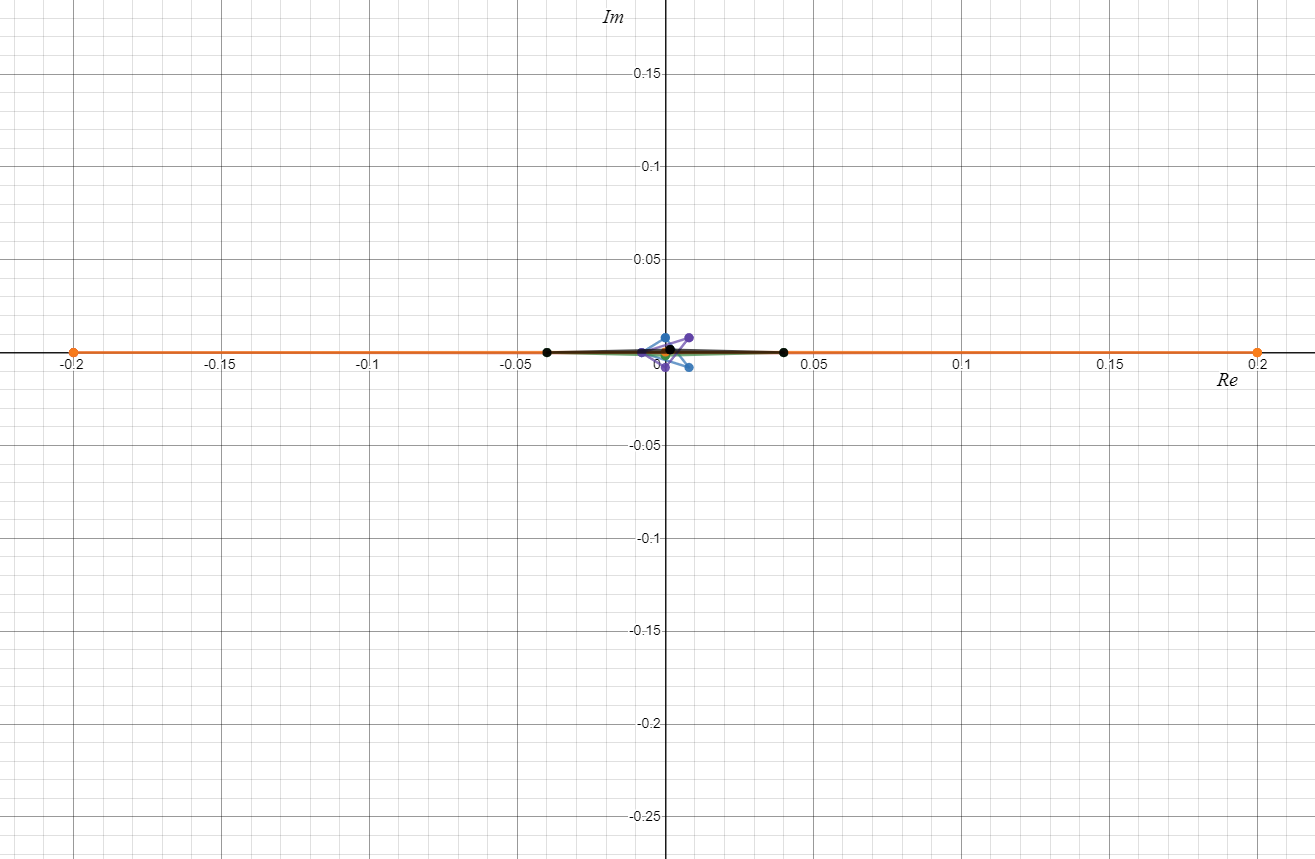
\includegraphics[scale=0.3]{unitaryTriangles}
		\centering
		\caption{The six triangles plotted for $A=\rho=\eta=1$ and $\lambda=0.2$}
		\label{fullPlot}
		\centering
	\end{figure}
	
	
	\begin{figure}[h]			
		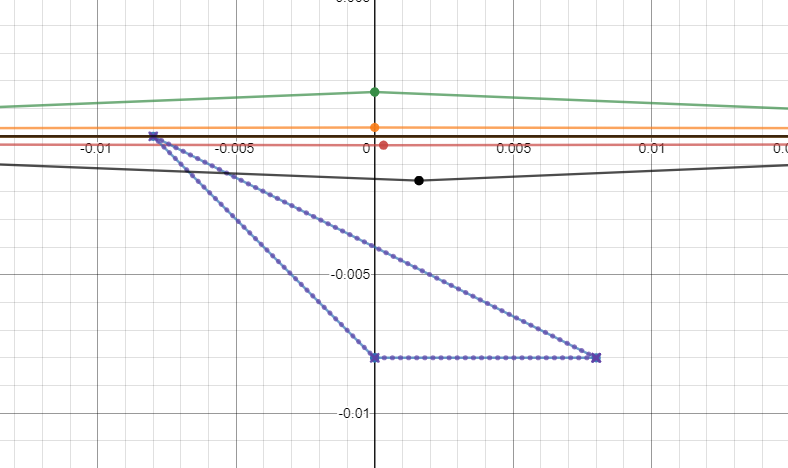
\includegraphics[scale=0.3]{unitaryTrianglesZoom}
		\centering
		\caption{The six triangles plotted to better see the two triangles whose sides are of similar size}
		\label{zoomPlot}
		\centering
	\end{figure}
	
	\textbf{Part b}
	\\
	Show that to leading order in $\lambda$ the two remaining triangles are really the same triangle. 
	\\
	\\
	\textbf{Solution}
	\\
	To leading order in $\lambda$, we can write the 
	\\
	\textbf{Part c}
	
\end{homeworkProblem}


\end{document}
